
%    INSTITUTE OF PHYSICS PUBLISHING                                   %
%                                                                      %
%   `Preparing an article for publication in an Institute of Physics   %
%    Publishing journal using LaTeX'                                   %
%                                                                      %
%    LaTeX source code `ioplau2e.tex' used to generate `author         %
%    guidelines', the documentation explaining and demonstrating use   %
%    of the Institute of Physics Publishing LaTeX preprint files       %
%    `iopart.cls, iopart12.clo and iopart10.clo'.                      %
%                                                                      %
%    `ioplau2e.tex' itself uses LaTeX with `iopart.cls'                %
%                                                                      %
%%%%%%%%%%%%%%%%%%%%%%%%%%%%%%%%%%
%
%
% First we have a character check
%
% ! exclamation mark    " double quote  
% # hash                ` opening quote (grave)
% & ampersand           ' closing quote (acute)
% $ dollar              % percent       
% ( open parenthesis    ) close paren.  
% - hyphen              = equals sign
% | vertical bar        ~ tilde         
% @ at sign             _ underscore
% { open curly brace    } close curly   
% [ open square         ] close square bracket
% + plus sign           ; semi-colon    
% * asterisk            : colon
% < open angle bracket  > close angle   
% , comma               . full stop
% ? question mark       / forward slash 
% \ backslash           ^ circumflex
%
% ABCDEFGHIJKLMNOPQRSTUVWXYZ 
% abcdefghijklmnopqrstuvwxyz 
% 1234567890
%
%%%%%%%%%%%%%%%%%%%%%%%%%%%%%%%%%%%%%%%%%%%%%%%%%%%%%%%%%%%%%%%%%%%
%
\pdfminorversion=4

\documentclass[12pt]{iopart}
\usepackage{graphicx}
\usepackage{amssymb}
\usepackage{enumitem}
\usepackage{xcolor}
\newcommand{\gguide}{{\it Preparing graphics for IOP Publishing journals}}
%Uncomment next line if AMS fonts required
%\usepackage{iopams}  
\begin{document}

\title[]{\textcolor{red}{NOT READY FOR REVIEW} Detection of target object recognition in simulated driving}

\author{R Aydarkhanov$^1$,
M Uscumlic$^2$,
L Gheorghe$^2$,
R Chavarriaga$^3$,
J d R Millan$^4$}


\address{$^1$EPFL, Switzerland}
\address{$^2$EPFL, Switzerland}
\address{$^3$EPFL, Switzerland}
\address{$^4$TU Austin, USA}
\ead{ruslan.aydarkhanov@epfl.ch}
\vspace{10pt}
%\begin{indented}
%\item[] August 2017
%\end{indented}

\begin{abstract}
\end{abstract}

%
% Uncomment for keywords
\vspace{2pc}
\noindent{\it Keywords\/}: Brain-computer interfaces, Electroencephalography, Eye tracking, Driving
%
% Uncomment for Submitted to journal title message
%\submitto{\JPA}
%
% Uncomment if a separate title page is required
%\maketitle
% 
% For two-column output uncomment the next line and choose [10pt] rather than [12pt] in the \documentclass declaration
%\ioptwocol
%



%There exist various well-established EEG-based BCI paradigms which
%provide a high performance and rely on such phenomena as
%Sensorimotor Rhythms (SMR), Steady-State Evoked Potentials (SSEP),
%or Event-Related Potentials (ERP) and others \cite{hwang_eeg-based_2013}.
%For each paradigm a specific data processing and feature
%extraction steps are required \cite{lotte_review_2018}.

\section{Introduction}
\label{sec:intro}

We study decoding of neural and behavioral correlates 
of visual recognition in simulated driving.
%Driving is a good example of daily activity in real life
%where BCI can enhance the driver's experience.
Driving is a complex activity involving a range of neural processes from motor control
to visual information processing, thus illustrating
many BCI challenges in real world application.

There are many examples in literature where EEG signature
of visual recognition was reported.
In the controlled experiments where subjects had to recognize
rare target stimuli in the sequence, the recognition process
is reflected in EEG as a well-known P300 Event Related Potential (ERP).
It was successfully used in various BCI applications such as
P300-based speller because of high decoding performance.
With the typing speed of 10 characters per minute \cite{rezeika_braincomputer_2018},
the home use of such spellers can improve the quality of life
of patients with strong motor disabilities, such as ALS \cite{sellers_brain-computer_2010,holz_long-term_2015}.
For healthy users, however, this setup and typing performance does not bring any value.

Successful decoding of visual recognition in free viewing tasks
would open space for BCI application for healthy users.
In free viewing conditions people need to fixate
or track moving objects to perceive it in all details.
Fixations evoke a type of ERP called Eye Fixation Related Potentials (EFRP)
and some studies showed that later components of EFRP resemble P300
component from oddball paradigm.

Visual stimuli mostly used in these studies range from simple geometric shapes
randomly positioned in static scenes and natural images to synthetic dynamic
scenes \cite{}. Only a few attempts on EFRP decoding in videos or VR simulations
have been reported \cite{}. \textcolor{red}{Limitations of these studies
and motivate my study.
Explain that the used experimental conditions do not correspond to real world environment.
There is no real driving involved as a primary task STUDY 1.
The authors sped up the action video to clearly define the relevant
event time STUDY 2.}

In our study subjects perform visual recognition task while primarily engaged
in driving in a car simulator.
The subject are faced with natural radially expanding optic flow.
We study EFRP
while driving
facing optic flow
yet we ensured that recognition happens upon the fixation by introducing pop up effect.
Otherwise, there would be 2 challenges: 
1) case when driver gazes at the distant object
until he approaches it close enough to recognize and
2) case when he returns gaze to the object multiple times until the object
is recognizable.
The latter challenges collecting clean data while the former challenges
the EFRP decoding itself.




%Brain Computer Interfaces (BCI) proved their potential utility 
%by successfully passing tests in controlled laboratory conditions.
%One of the remarkable examples is P300-based spellers
%which allow to type up to 10 characters per minute \cite{rezeika_braincomputer_2018}.
%The home use of such spellers can improve the quality of life
%of patients with strong motor disabilities, such as ALS \cite{sellers_brain-computer_2010,holz_long-term_2015}.
%However, bringing BCI to everyday life for healthy people
%remains a challenge.

%A classical P300-based speller presents a static matrix of symbols on a screen.
%The symbols are highlighted in groups (i.e. column-wise and row-wise)
%by flashing regularly. The users pay attention on the screen and 
%do a mental evaluation of whether the target symbol is highlighted or not.
%At each flash an Event-Related Potential (ERP)
%is elicited, and when the user believes that the target is active
%the ERP will contain P300 component.
%To reduce the noise in the signals the users are instructed to limit their body as well as
%eye movements by staring in the middle of the screen.

%The real world is more diverse and more dynamic than traditional
%P300-based experimental protocols. So the time to evaluate
%the visual input can vary which is reflected in the ERP waveform \cite{arico_evaluation_2013}.
%Numerous attempts were done to close this gap and investigate
%the limitations to detect P300 under more challenging conditions
%which includes recognition of dynamic or semantically
%rich stimuli as compared to alphabet characters \cite{rosenthal_evoked_2014}.
%Additionally, natural environment does not provide regular flashing stimulation.
%Instead, it is sampled by free visual exploration with free eye movements.
%There are three major types of eye movements: saccades, fixations
%and smooth pursuit. The clear and sharp perception of visual input
%is only possible during fixations and smooth pursuit.
%Fixations trigger a type of ERP called Eye Fixation Related Potentials (EFRP).
%Although P300 was successfully detected within EFRP,
%it 


%P300 is a reflection of a cognitive process of stimulus evaluation and
%categorization. Its application has potential to go beyond the selection from 
%a limited set of stimuli. P300 can be monitored and detected during execution
%of everyday tasks. For example, driving a car provides a suitable context
%for this type of BCI application. Detection of recognition of critical objects
%or traffic events will give a valuable information for the Advanced
%Driving Assistant Systems (ADAS). Various paradigms were developed
%to investigate decoding performance of EFRP-based P300 during simulated driving.
%For passive driving task which require only brake input from the driver
%the P300 decoding can achieve above chance level for half of the participants \cite{jangraw_neurally_2014}.
%In this paper we address the P300 decoding during active simulated driving with automatic gear.




\section{Materials and Methods}
\label{sec:methods}

\subsection{System}
Our system is based on the driving simulator previously used for
EEG-based BCI experiments \cite{khaliliardali_action_2015,zhang_eeg-based_2015}.
We extend the protocol published in \cite{renold_eeg_2014}.
It allows for immersive driving experience through the utilization
of real Nissan driving chair with steering wheel and two pedals (gas and brake).
The visual input is provided with three 3D monitors which create multiple renders for
different angles. The virtual environment is implemented on a basis of
the open source driving simulator project VDrift \cite{noauthor_about_nodate}.
The environment resembles a regular grid city with static objects, i.e.
building, traffic lights, fields. The task-related objects include
direction indications on the road, target cue, boards with symbols
and finish lines. 

\subsection{Tasks}
The experimental session is completed in 2 phases: offline and online
The instructions were similar for both phases.
First of all, it is necessary to drive through the city while
following the direction indications.
Every road begins and ends with a left or right turn at the crossing.
Within each road subjects perform the cognitive task while driving.
In the beginning of the road the target symbol (the cue) is depicted
on the road. Subjects must look at the cue and remember it.
While driving trough the road multiple boards appear one by one
on both sides of the road. Only a fraction of the boards have
the target symbol on them. Subjects must visually attend all the boards
and count the number of boards with the target symbol. 
The terminal part of the road is marked with a finish line and 
reserved for the reporting in offline or feedback in online protocols.

\subsubsection*{Offline.}
The steering is equipped with a button.
After crossing the finish line the subject presses the button as many times
as the number of target boards he/she counted along the current road.
\subsubsection*{Online.}
In the online scenario the system decodes the target based
on the neural responses of the subject. 
After crossing the finish line the predicted target is projected
at the bottom of the screen. Subjects are instructed to pay
attention to this feedback.

One quarter of the roads are designed empty to allow subjects to rest.

\subsection{Stimuli presentation}

The board presentation is carefully adjusted to guide the behavior of subjects.
First of all, boards are invisible unless the driver approaches them
close enough making them to pop up suddenly.
Their positions are generated using the following rules.
The boards appear on a regular grid along the road however
randomly on either side of the road with maximum of 2 boards
on the same side in a row. The number of boards on left
and right sides are balanced. Since the pop up distance was greater
than the distance between the boards along the road, multiple
boards from the same side were visible in the same time
so their horizontal and vertical position were adjusted to avoid
the overlap for the driver view.

The maximum speed of the car was limited to ensure that all the targets
can be attended. The subjects were allowed to slow down if it is necessary
to attend all the boards and count the targets.
Nonetheless, all the subjects practiced until they felt comfortable 
with completing the recognition task at the maximum speed
during the EEG setup.
Due to constant speed and regular placement of the boards they
popped up at a regular pace with 900 ms period.

In order to link the perception of the symbols on the board
with the eye fixations, the recognition by
peripheral vision must be avoided. Therefore, the target and distracting
symbols were similar and surrounded by \# character.
Additionally, we added a bright red border around the board similar 
to the traffic signs
to create a contrast with the environment and facilitate
their identification.

\subsubsection*{Offline.}
In the offline phase one of the two symbols were depicted on each board:
E and horizontally flipped E.
One of them was randomly chosen as a target and were presented as the cue
at the beginning of the road. There were 2-5 targets out of 12 boards
on each road with the average fraction of targets of 0.25 in total.
\subsubsection*{Online.}
In the online phase 4 different symbols were available. There were
3 boards of each type resulting into 12 boards on the road.
Only one of them was a target on each road.


\subsection{Data collection}
We had 13 volunteers (N male and N female) with the average age of N.
They participated in one 3 hour session which included
1 hour of the set up, ~45 minutes per phase and ~30 minute break in between.
The offline phase consisted of 3 runs through the city  whereas the online
phase could have from 3 to 5 runs depending on the available time.
One run included 20 non-empty roads with 240 boards in total.
Before each run the subjects were asked to move their eyes up-down and left-right
for one minute in order to collect the data for eye movement artifact removal.

The EEG was acquired with BioSemi ActiveTwo system with 64 electrodes at 2 kHz sampling rate.
Additionally, we recorded 3 EOG channels to collect the eye movement data:
two electrodes next to the outer canthi of the eyes and one above the nasion.
The EEG data were captured and saved on the laptop. The real time processing
of EEG in online phase was done on the same laptop using CNBI loop.

The eye gaze was recorded with SMI RED Eye tracking system with the sampling rate of 120 Hz.
The chair and eye tracker positions were adjusted for each subject. The eye tracker
was calibrate with 13 points only once after the EEG setup and before beginning of 
the experiment.

The driving simulator logged various information of the driver location,
the controllers state and the 2D position of boards on the screen at the sampling rate
of 256 Hz. In order to synchronize the data acquisition on three separate machines
(EEG, eye tracking and driving simulator) at different sampling rates,
a square pulse of 4 Hz was generated by the driving simulator and sent 
to the eye tracker through TCP connection and to BioSemi through the parallel port.



\begin{figure}[!t]
    \includegraphics[trim={0cm 0cm 0cm 0cm},clip,width=0.6\columnwidth]{../images/Driving-photo.jpg}
    \caption{Experimental setup.}
\label{fig:setup}
\end{figure}

\subsection{Fixation extraction and analysis}
There exist numerous methods to extract eye movement events
from the eye gaze direction. Some of them proved to provide
a better quality according to the human experts
however are more challenging to implement in real time.
We used different methods for offline and online.
Simulated online analysis is implemented identical to online phase.


\subsubsection*{Offline.}
The detection of fixation is done with the Identification by 2-Means Clustering (I2MC) method.
We relied on the implementation provided by the authors of the method
using the default parameters.
The main idea behind is to find the transition between two consecutive fixations
by applying 2-mean clustering in a sliding window manner.
During fixation the eyes do not move so if we can clearly detect
2 clusters it means that they correspond to two fixations.
This method is more precise and robust to noisy outliers which
allows to obtain a training dataset of higher quality.

\subsubsection*{Online and simulated online.}
We could not use the provided implementation of I2MC in real time
to extract fixations so we used the Identification by Dispersion-Threshold (IDT)
supplied with our eye tracking system. Fixation in IDT is extracted
when the signals lies within the dispersion thresholds for at least a minimum fixation duration.
It requires two parameters: we used 100 ms for the minimum fixation duration
and 200 pixels for the maximum dispersion.

The cognitive response is stronger when the stimulus is perceived and recognized
for the first time. We assume that subjects categorized the symbol at the first
attendance so we use only the first fixations on the boards for our analysis.

The visual input during the task is dynamic. Due to driving through
the virtual environment the objects including the boards are also moving on the screen.
So we assume that most of the board attendances are done with
smooth pursuit rather than fixations. 
To the best of our knowledge there is no available algorithm for efficient
extraction of smooth pursuit for eye movement data sampled at 120 Hz.
The only consequence of 
extracting fixation from smooth pursuit is that a single smooth pursuit
may be oversegmented into multiple fixations.
For the sake of our analysis we do not need to differentiate between
fixations and smooth pursuit movement. The onset of first fixation on a board
will coincide with the onset of smooth pursuit.

For the behavioral analysis we estimate the total attendance time of boards
for the first uninterrupted visit or dwell time. The dwells were created
by merging all the fixations on the same board with saccade durations
between them below 50 ms.

Each fixation and dwell were assigned to a target board, a non-target board or non-board.
Due to a reading visual span of several degrees, the board movement and 
noisy eye tracking data we applied the following approach to assign the boards
to fixations. For each eye gaze sample we estimate the probability of
fixating eyes on the center of the board according to a normal distribution.
After averaging log-probabilities across the dwell time we apply a hard
threshold to assign the fixation to a board or a non-board class.


\subsection{EEG data processing}
All the EEG and EOG were filtered with Butterworth band-pass filter
of order 4 within the band [1, 10] Hz
forward and backward and downsampled from 2 kHz to 256 Hz.
Due to low conductivity of the skull and the skin,
EEG signal is spatially smoothed so a high contrast between nearby channels
is a result of noise and movement artifacts. We remove this noise
by keeping only low spatial frequency components after decomposition EEG with SPHARA.
Horizontal and vertical components of eye movement were estimated which allowed
to remove the eye movement artifacts from EEG using multivariate regression.
The coefficients of multiple regression were estimated from the 
one-minute session of eye movements before the corresponding run.
Then the signal is spatially
filtered with common-average-reference (CAR). The epochs are extracted
from time window of [200, 1000] ms after the fixation onset.
We investigate and compare different sets
of features, which include EFRP waveform and covariance-based features.

\subsubsection*{Offline.}
For the offline analysis we chose the following combination of features and classifiers:
\begin{itemize}
    \item Penalized logistic regression (PLR) trained on waveform features after reducing
        the dimensionality with PCA. Only the components which explain 90\% of variance
        are kept. 
    \item PLR trained on dwell time on the boards.
    \item PLR trained on the combination of waveform features with dwell time. We concatenate
        the two feature sets before applying PCA to keep 95\% of variance. Since the dynamic
        range of dwell time in ms is greater than the one of EEG in uV, most of the information
        remains is projecte
    \item Random forest trained on waveform features. We use 100 decision trees and
        with maximum depth of 5.
    \item PLR trained on Riemannian features from simple epochs.
        To build Riemannian features we
        estimate spatial covariance matrix with shrinkage and project it
        to the tangent space according to the classical Riemannian geometry on SPD matrices.
        We subselected 8 channels based on mean Fisher score across the epoch.
    \item PLR trained on Riemannian features from augmented epochs.
        Before computing the covariance matrix we augment the epoch with the averaged ERP
        for each class (target and non-target). Otherwise, it is identical to the previous
        approach.
\end{itemize}

Since PLR is a linear regularized classifier we standardize all the features to z-score when
using PLR.


\subsubsection*{Online.}
The online phase required the real time processing. SMI system provides
a real time eye fixation detection. The fixations were buffered
by a parallel process within the driving simulator, matched with the boards,
and a trigger was sent to the BioSemi system 3 s after the onset of each the fixation
on a board. We choose 3 s delay because we apply non-causal filter on EEG data.
EEG processing  was identical to the offline procedure
except for 2 steps:
\begin{itemize}
    \item the spectral filtering was done on a 5 s buffer of data,
        approximately around [-2, 3] s around the fixation onset;
    \item the eye movement artifacts were removed based on the multiple
        regression coefficients trained with offline phase eye movement data.
\end{itemize}
On the data obtained in the offline phase we trained Random Forest classifier
and applied it in real time. The probability for the target class was sent
back to the driving simulator. After crossing the finish line
the probabilities were averaged per each symbol (1 out of 4).
The symbol which had the highest probability of being a target was
shown to the subject on the screen.

\subsubsection*{Simulated online.}
The EEG processing was identical to the offline analysis
except for the eye movement artifacts removal. The multiple regression
model was obtained from offline data.

\subsection{Performance estimation}

Performance is estimated differently for the data from offline and online
phases.
\subsubsection*{Offline.}
We employ nested cross validation to adjust various hyperparameters in the inner loop:
regularization term for PLR and the tree depth in Random Forest.
The purpose of the outer loop is to obtain an unbiased performance estimation
so it is critical to avoid training and testing on correlated data.
We achieve it by performing leave-one-run-out for the outer loop,
although we had only 3 offline runs.
The inner loop is implemented with 4-fold cross validation while keeping
the temporal order of the trials before the split.
Since the classes of target and non-target eye fixations are unbalanced,
we utilized AUC to measure the classification performance.

\subsubsection*{Simulated online.}
After training the classifiers on the offline data we applied them 
to the online data and assessed AUC.

\subsubsection*{Online.}
During online phase we predicted the target symbol from the EFRP classification.
We assess the overall performance with accuracy and confusion matrices
for 4 symbols.

\section{Results}
\label{sec:results}
\subsection{Behavioral analysis}

\subsubsection*{Board attendance}
Subject attended most of the boards in the offline phase and only
half of them in the online phase. The average attendance rate
is shown in the Table \ref{tab:boardAtt}.
Repeated measures ANOVA shows significant difference between
all 4 groups: targets in offline, targets  in online,
non-targets in offline and non-targets in online, with $p-value < 0.0001$.
Post-hoc analysis shows that it is driven by the difference between
offline and online phases with p-value $< 0.0001$ (paired t-test).
The difference between targets and non-targets is not significant with p-value $= 0.03$
so we can assume that subjects could not differentiate the symbols
with peripheral vision.

\begin{table}
    \centering
    \caption{Board attendance rate}
    \begin{tabular}{c | c | c}
        \hline 
        & Offline & Online \\
        \hline 
        Targets & 0.87 & 0.45 \\
        Non-Targets & 0.87 & 0.43 \\
        \hline 
    \end{tabular}
    \label{tab:boardAtt}
\end{table}
%TargOff    0.868838
%DistOff    0.865138
%TargOn     0.454746
%DistOn     0.428700

\subsubsection*{Counting}
The total number of targets in offline phase is 173.
We analyzed the button presses which should be equal to the number of targets
on each road.
The average number of incorrect counts (both missed and extra counts) was 5,
the worst performance was at 15 errors (Figure \ref{fig:classAll}).


\subsubsection*{Dwell time}
We analyzed the distribution of dwell times on targets vs non-targets
in offline and online phases (Figure \ref{fig:dwell}). 
Most of the dwells are limited to the time between the boards pop up equal to 900 ms.
The dwell times are identical for non-targets in both phases and significantly
shorter than for targets (p-value $< 0.0001$).
The median dwell time for targets is significantly longer in online phase (p-value $< 0.0001$).

\begin{figure}[!t]
    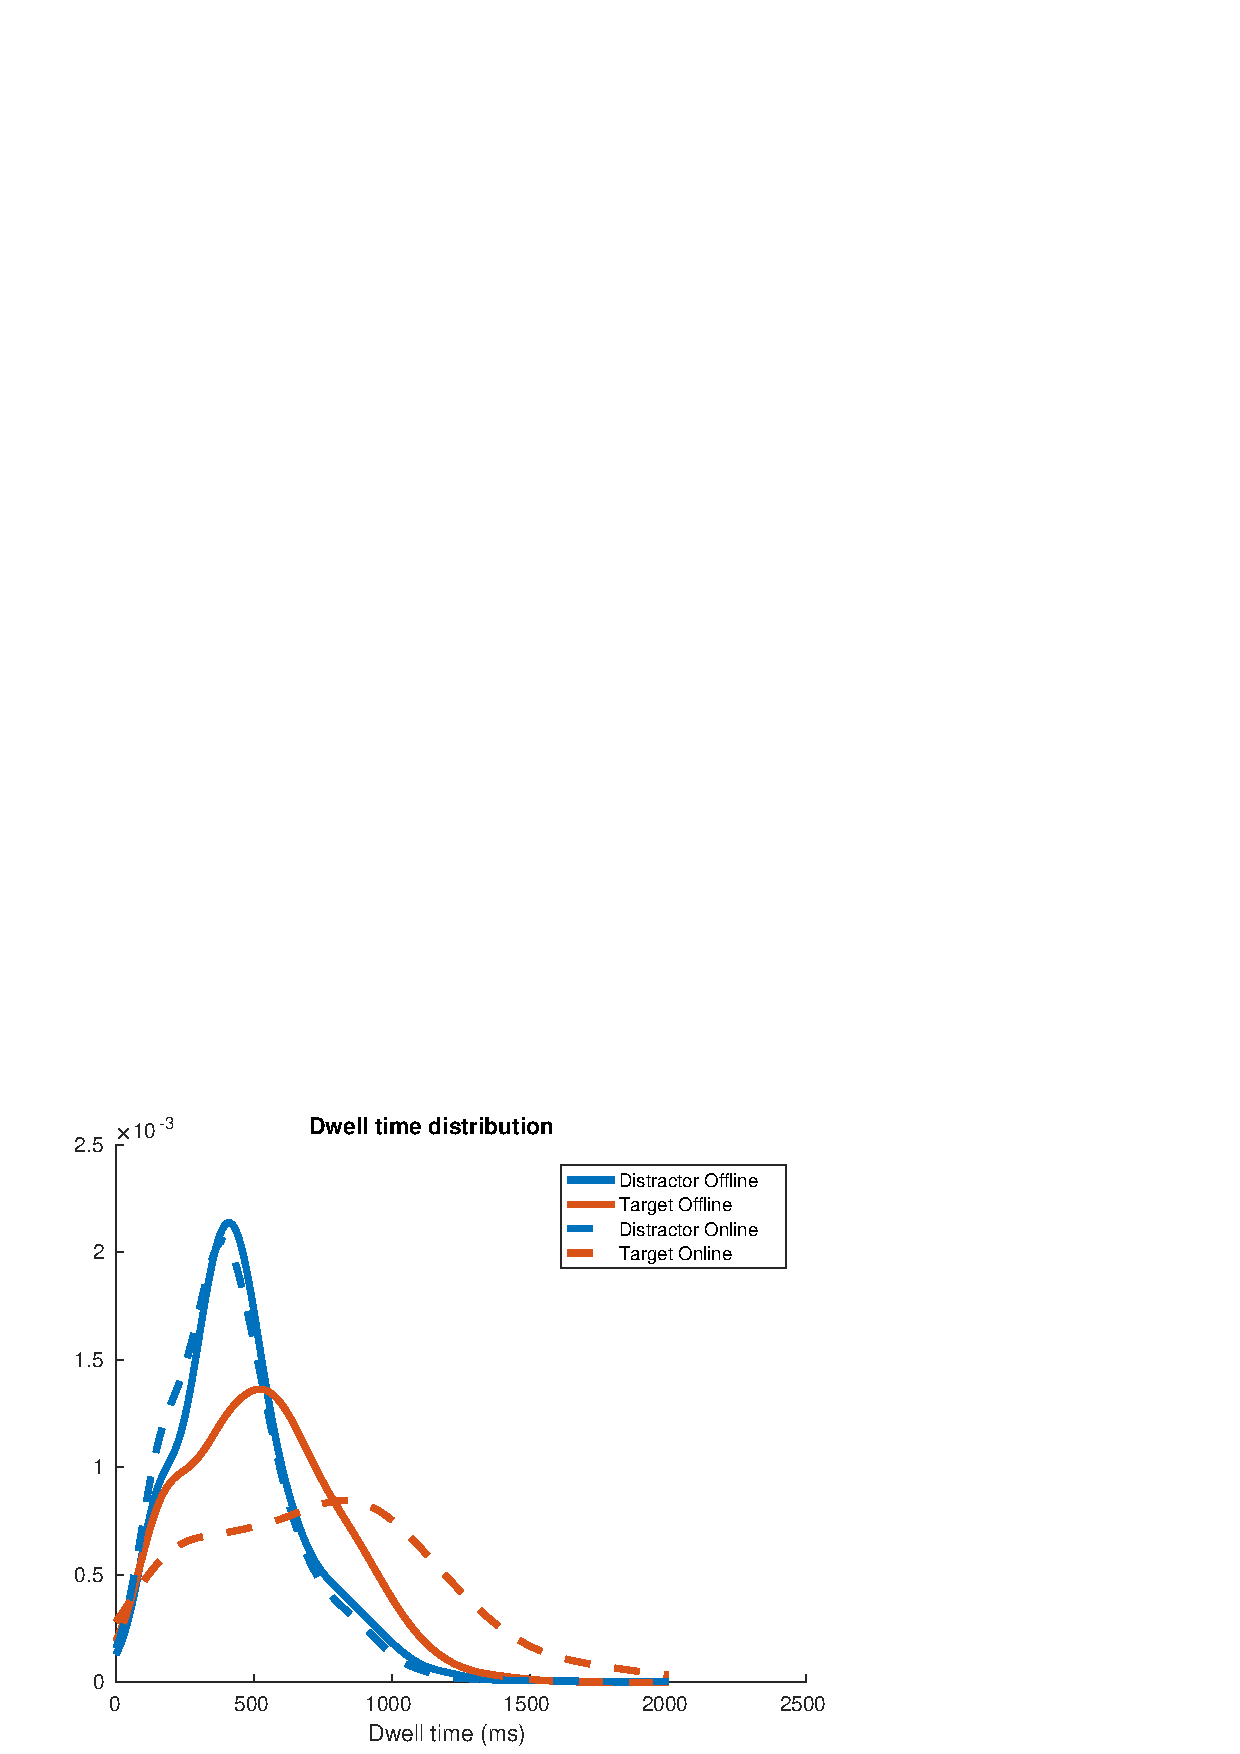
\includegraphics[trim={0cm 0cm 0cm 0cm},clip,width=0.6\columnwidth]{../images/DwelltimeDist_online_allmean.pdf}
    \caption{Dwell time distribution for targets vs distractors in offline and online phases.}
\label{fig:dwell}
\end{figure}

\subsection{ERP waveform}

\subsection{Comparison of decoding approaches}

\begin{figure}[!t]
    \includegraphics[trim={2cm 0cm 2cm 0cm},clip,width=1.1\columnwidth]{../images/ClassificationAll.png}
    \caption{Performance of EFRP classification with various approaches in offline analysis (top)
    and simulated online analysis (bottom). Each dot shows single fold performance
    in a leave-one-run-out cross validation for the corresponding classification approach.}
\label{fig:classAll}
\end{figure}

\subsubsection*{Offline}
All the classification approaches lead to the performance between 53 and 60 AUC points on average
(Figure \ref{fig:classAll})
which is statistically significant against random level of 50 
(p-values $< 0.001$ with Student's t-test after Bonferroni correction).
8 out of 13 subjects achieve performance above 60 for at least one of the approaches based
on neural correlates.
Although each subject has a different preferred approach, the differences between
the approaches are not statistically significant (p-value $= 0.16$ with repeated measures ANOVA).
It is worth noticing that the combination of both dwell time and EEG waveform is not always
better than just one of these feature sets.

\subsubsection*{Simulated online}
First of all, we note that the performance of neural-based approaches 
on online data is consistent with the training performance on offline data.
The average AUC values lie between 56 and 59 for each approach
which is statistically significant against 50
(p-values $< 0.001$ with Student's t-test after Bonferroni correction).

For approaches relying on the dwell time, however, the performance drastically improved
for multiple subjects. The average AUC for \textit{dwell} classifier increased
from 56 to 73 and for the \textit{Linear with Dwell} classifier from 59 to 67.
This improvement is a direct consequence of the changes in target dwell time
together with the constant non-target dwell time shown in \ref{fig:dwell}.


\subsection{Online performance}

\begin{figure}[!t]
    \includegraphics[trim={0cm 0cm 0cm 0cm},clip,width=0.5\columnwidth]{../images/OnlineConfusion.png}
    \caption{The aggregated confusion matrix of online decoding for each type of symbol being
    a target.}
\label{fig:onlineconf}
\end{figure}


\begin{table}
    \centering
    \caption{Online performance}
    %\tiny
    %\footnotesize
    \scriptsize
    \renewcommand{\arraystretch}{1.5}
    \begin{tabular}{l r r r r r r r r r r r r r}
        \hline
        Subjects & S1 & S2 & S3 & S4 & S5 & S6 & S7 & S8 & S9 & S10 & S11 & S12 \\
        \hline

        Accuracy & 0.44 & 0.38 & 0.45 & 0.29 & 0.44 & 0.35 & 0.39 & 0.25 & 0.31 & 0.38 & 0.38 & 0.4 \\ 
        %0.44, 0.38, 0.45, 0.29, 0.44, 0.35, 0.39, 0.25, 0.31, 0.38, 0.38, 0.4
        \shortstack{Accuracy \\ test} & \textbf{0.003} & 0.29 & \textbf{0.002} & 5.27 & \textbf{0.003} & 0.62 & 0.08 & 12.0 & 2.40 & 0.29 & 0.29 &
        0.16 \\
        \shortstack{Independence \\ test}  & \textbf{ 0.004} & 2.58 & 0.06 & 8.91 & 0.24 & 0.84 & 0.39 & 4.13 & 5.26 & 1.14 & 1.53
        & 2.07 \\
        \hline
        %Binom:  [0.003, 0.2903, 0.0016, 5.2731, 0.003, 0.6192, 0.0771, 12.0, 2.4047, 0.2903, 0.2903, 0.1592]
        %Chi * 12  [0.0044, 2.5806, 0.0608, 8.9126, 0.243, 0.8449, 0.3913, 4.1269, 5.2593, 1.1424, 1.5352, 2.0768]
    \end{tabular}
    \label{tab:onlineperf}
\end{table}

We assessed the task performance of each subject as the accuracy of
target decoding (Table \ref{tab:onlineperf}). The averaged accuracy 
equals 0.37 and it is significantly different from random level of 0.25 for
a classification of 4 between balanced classes (p-value $< 0.0001$ with Student's t-test).
Additionally, we applied statistical test to assess the accuracy per subject.
After Bonferroni correction only 3 subjects showed statistically better than random performance.

To verify the independence of the 4 classes in online phase
we computed the aggregated confusion matrices of across all symbol (Figure \ref{fig:onlineconf}).
We applied an independence test for confusion matrices per subject.
After Bonferroni correction only one subject.


\section{Discussion}
\label{sec:discussion}

In the online phase subjects looked longer on targets compared to the offline phase.
Although the subjects dwell time was not decoded directly, they were aware
that they could potentially influence the decoding quality. This might
lead to deliberate or unconscious changes in their behavior.


\section*{References}

\bibliographystyle{unsrt}
\bibliography{ObjRec_DS.bib}

\end{document}

